\section{Кубит на нейтральных атомах $^{87}\text{Rb}$}
\label{sec:chapter_2}

\subsection{Охлаждающие переходы}


\subsection{Массив оптических пинцетов}
% Про сортировку и перемещение можно полностью в массиве оптических пинцетов написать

Одним из преимуществ платформы на нейтральных атомах является то, что из атомов, в которые кодируется кубит, можно формировать произвольные одномерные и двумерные структуры, а также легко переключаться между ними. Делается это с помощью пространственного модулятора света(SLM) и акустооптического дефлектора(АОД) в скрещенной конфигурации. SLM представляет собой прямоугольную матрицу из жидких кристаллов, на каждый кристалл которой можно независимо подавать напряжение и, тем самым, менять показатель преломления за счёт эффекта двулучепреломления. Таким образом, с помощью SLM можно формировать произвольную фазовую маску(голограмму), ограниченную лишь размерами матрицы и размером пикселя. С помощью голограммы можно преобразовать падающий на неё лазерный луч в двумерный массив оптических пинцетов произвольной конфигурации, в который далее можно загрузить атомы. Сами фазовые маски можно рассчитать с помощью алгоритма Герчберга-Сакстона \cite{Gerchberg1972APA} и его модификаций \cite{robust_masks,Zupancic:16}.

\textcolor{red}{Надо добавить картинку импульсной последовательности, фотографии атомов в оптическом пинцете, а также картинку фазовой голограммы на SLM.}

Для загрузки Атомы из МОЛ перегружаются в двумерный массив оптических пинцетов \cite{Ashkin:99}, сформированный жёстко-сфокусированными гауссовыми пучками с радиусом перетяжки порядка $1 \text{ мкм}$. Если использовать оптические пинцеты в режиме столкновительной блокады\cite{Schlosser_Grangier,Kuppens_Wieman}, при которой сильно возрастают двухчастичные потери, то при загрузке атомов из МОЛ в дипольной ловушке примерно с одинаковой вероятностью оказывается либо один атом, либо ноль. Этот механизм позволяет ловить одиночные атомы, а затем кодировать в них кубит. 



\subsection{Инициализация состояния}

Чтобы что-то делать с кубитами, нужно уметь инициализировать их начальное состояние. В нашей системе в качестве кубитных состояний используются магнитные подуровни сверхтонкого расщепления основного состояния $^{87}\rm{Rb}$, $\ket{0}=\ket{5^2S_{1/2},F=1,m_F=0}, \; \ket{1}=\ket{5^2S_{1/2},F=2,m_F=0}$, поэтому нам нужно уметь помещать атом в одно из этих состояний. Для инициализации используется схема, показанная на рисунке \ref{fig:initialization}.

\begin{figure}[ht]
	\centering
	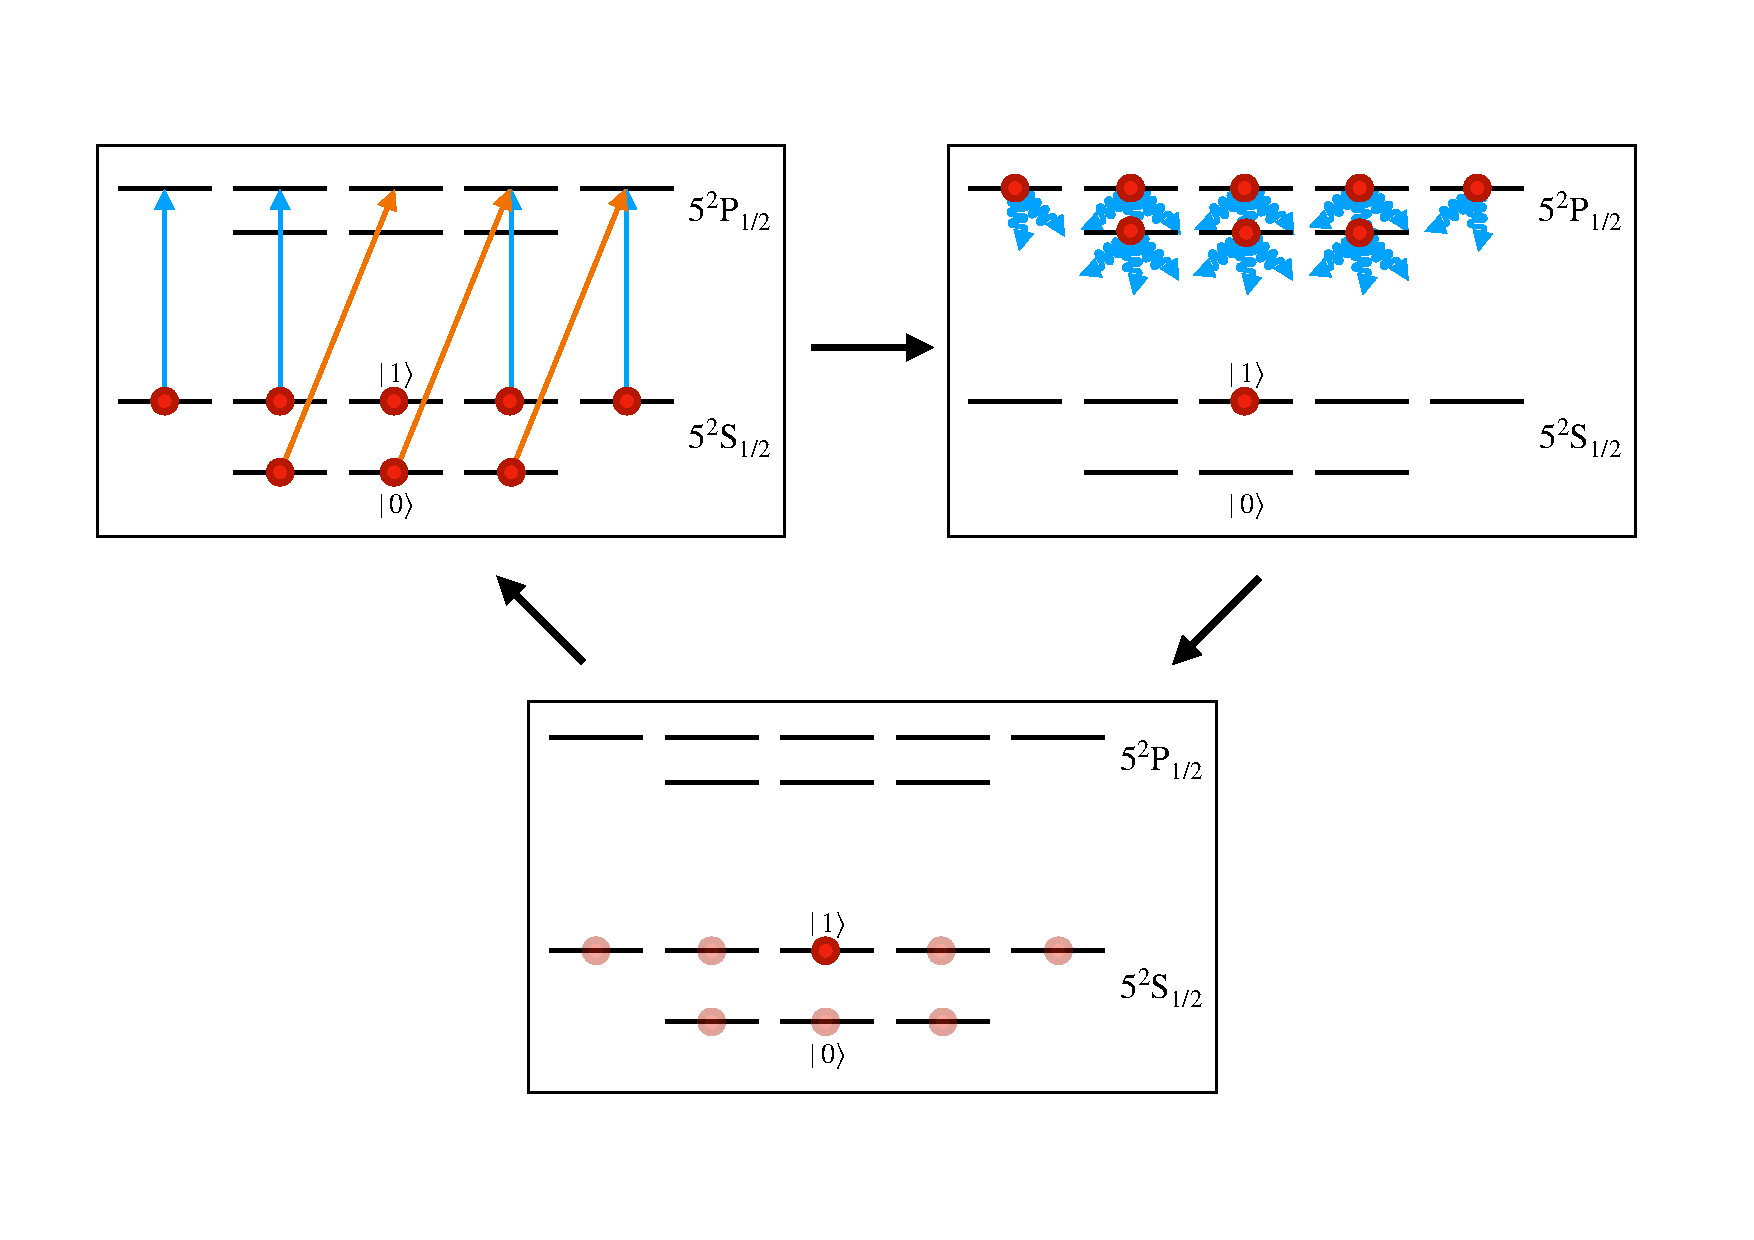
\includegraphics[width=0.9\textwidth]{images/initialization_scheme.pdf}
	\caption{Населённость с уровня $\ket{1}$ не уходит на другие уровни, так как переход $\ket{5^2\rm{P}_{1/2},F=2,m_F=0}\leftrightarrow \ket{5^2\rm{P}_{1/2},F=2,m_F=0}$ запрещён правилами отбора для дипольных переходов, поэтому вся населенность в итоге сваливается на уровень $\ket{1}$.}
	\label{fig:initialization}
\end{figure}

С помощью двух лазеров с линейной и правой циркулярной поляризацией атомы из терма $5^2\rm{S}_{1/2}$ с $m_F\neq0$ перекачиваются на терм $5^2\rm{P}_{1/2}$, а затем спонтанно распадаются обратно на $5^2\rm{S}_{1/2}$, причем часть населенности попадает на уровень $\ket{1}=\ket{5^2\rm{S}_{1/2},F=2,m_F=0}$. Так как переход $\ket{5^2\rm{P}_{1/2},F=2,m_F=0}\leftrightarrow \ket{5^2\rm{P}_{1/2},F=2,m_F=0}$ дипольно-запрещён правилами отбора по чётности \cite{Belousov} \textcolor{red}{(вроде, по чётности, но это неточно)}, то населённость с него не уходит на терм $5^2\rm{P}_{1/2}$, а значит после нескольких итераций такой последовательности вся населенность останется на уровне $\ket{1}$. Естественная ширина и время жизни терма $5^2\rm{P}_{1/2}$ составляют примерно $\Gamma = 2\pi \times 6 \text{ МГц}$ и $170 \text{ нс}$ \cite{Rb87}, для накачки используется мощный пучок с $\Omega \gg \Gamma$, поэтому скорость инициализации начального состояния определяется временем жизни $5^2\rm{P}_{1/2}$. Чтобы минимизировать ошибку приготовления состояния, последовательность выполняется в течение $5 \text{ мс}$.


\subsection{Однокубитные логические операции}

Однокубитные логические операции производятся с помощью возбуждения осцилляций Раби в двухуровневой системе, образованной двумя выделенными энергетическими уровнями атома $^{87}\rm{Rb}$. Пусть уровни $\ket{0}$ и $\ket{1}$ отстоят по энергии на $\hbar \omega_0$, на атом светит переменное классическое поле с частотой $\omega$, тогда гамильтониан системы атом + поле в приближении вращающейся волны можно записать в виде(гамильтониан Раби, $\hbar=1$) \cite{Lukin, Steck}

\begin{equation}
	H = \frac{\Delta}{2} \sigma_z + \frac{\;\rm{Re}(\Omega)}{2}\sigma_x + \frac{\;\rm{Im}(\Omega)}{2}\sigma_y= \frac{1}{2}\vec{\Omega}\cdot\vec{\sigma},
\end{equation}

где $\Delta = \omega - \omega_0$ - отсройка от резонанса, $\Omega$ - частота Раби, которая выражается через матричные элементы соответствующего оператора из мультипольного разложения \cite{LL_teorpol,Steck}. $\sigma_i$ - матрицы Паули, которые в кубитном базисе выражаются как

\begin{equation}
	\sigma_x = \ket{0}\bra{1} + \ket{1}\bra{0}, \; \sigma_y = i\ket{1}\bra{0} - i\ket{0}\bra{1}, \; \sigma_z = \ket{0}\bra{0}-\ket{1}\bra{1}.
\end{equation}

Оператор эволюции записывается в виде 

\begin{equation}
	U(t) = \exp\left(-\frac{it}{2}\vec{\Omega}\cdot\vec{\sigma}\;\right) = \exp\left(-i\frac{\tilde{\Omega}t}{2}\vec{n}\cdot\vec{\sigma}\right),
	\label{eq:evolution_operator}
\end{equation}

то есть мы получили вращение на сфере Блоха на угол $\tilde{\Omega}t$ вокруг вектора $\vec{n}$, которые выражаются как

\begin{equation}
	\vec{n}=\left(\frac{\rm{Re(\Omega)}}{\sqrt{|\Omega|^2 + \Delta^2}},\frac{\rm{Im}(\Omega)}{\sqrt{|\Omega|^2 + \Delta^2}},\frac{\Delta}{\sqrt{|\Omega|^2 + \Delta^2}}\right),
\end{equation}

\begin{equation}
	\tilde{\Omega} = \sqrt{|\Omega|^2 + \Delta^2}.
\end{equation}

Отсюда сразу видно, что для экспериментальной реализации $X$ и $Y$ гейтов можно посветить на атом резонансным $\Delta = 0$ полем с фазой $0$ и $\pi/2$ соответственно в течение времени $t$ такого что $\Omega t = \pi$. Для реализации $Z$-гейта можно посветить на атом сильно-отстроенным пучком, 

Сейчас на нашей установке можно совершать однокубитные операции с помощью радиочастотного поля, возбуждающего магнитодипольный переход между кубитными состояними, либо с помощью оптических рамановских двухфотонных переходов. Рассмотрим для начала реализацию однокубитных гейтов с радиочастотным возбуждением.

\subsubsection{Однокубитные операции с СВЧ-возбуждением}

Одной из схем реализации однокубитных вентилей является использование резонансной СВЧ-антенны, которая возбуждает магнитодипольный переход между кубитными состояниями $\ket{0}=\ket{5^2S_{1/2},F=1,m_F=0}$, $\ket{1}=\ket{5^2S_{1/2},F=2,m_F=0}$ на частоте $6.8 \text{ ГГц}$. Так как СВЧ-излучение засвечивает сразу весь атомный массив (расстояние между атомами порядка $3$ мкм), то требуется дополнительный адресующий лазер для реализации локальных однокубитных операций(рис. \ref{fig:shf_scheme}). 

\begin{figure}[ht]
	\centering
	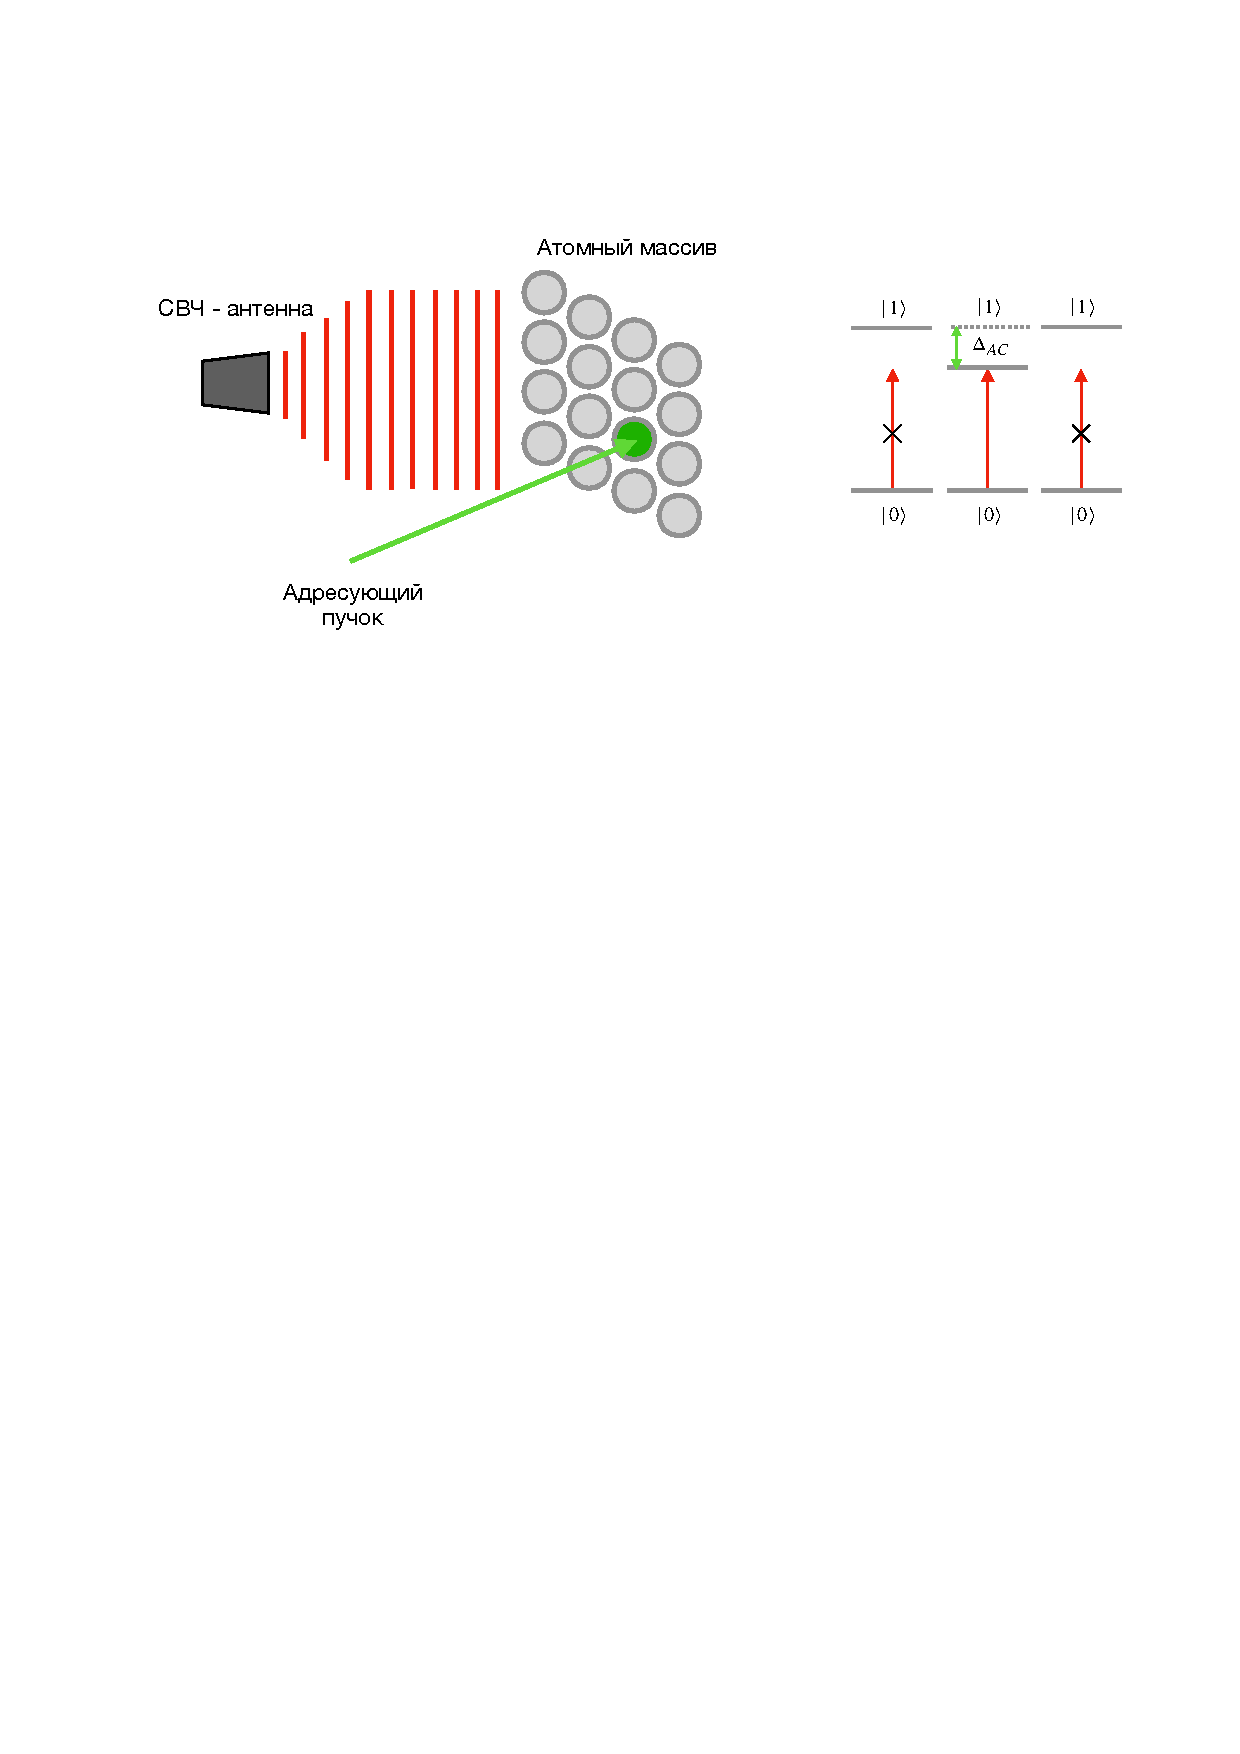
\includegraphics[width=0.8\textwidth]{images/shf_gates.pdf}
	\caption{Схема реализации адресных гейтов с помощью СВЧ-антенны и дополнительного адресующего лазера. Все атомы, кроме целевого, находятся вне резонанса с СВЧ-антенной. Целевой атом находится в резонансе за счёт оптических штарковских сдвигов от адресующего пучка.}
	\label{fig:shf_scheme}
\end{figure}

СВЧ-антенна отстраивается от кубитной частоты так, чтобы подавить осцилляции Раби на всех атомах. Для целевого же атома адресующий пучок сдвигает частоту перехода за счёт оптического штарковского сдвига(AC Stark shift), возвращаёт целевой атом в резонанс с антенной. Так реализуются локальные однокубитные операции с помощью СВЧ-антенны. К недостаткам локальных СВЧ-гейтов можно отнести их большую длительность за счёт делокализации излучения по всему массиву, нагрев атома за счёт мощного адресующего пучка. Таким образом, СВЧ-излучение больше подходит для реализации глобальных однокубитных операций сразу над всем атомным массивом, что тоже иногда требуется делать. 

На текущий момент точность глобальных СВЧ-гейтов составляет $F=(99.95 \pm 0.07)\%$. Оценка точности однокубитных операций производится с помощью протокола randomized benchmarking \cite{Hines_2023,Proctor:2022aa}. К факторам, ограничивающим точность СВЧ-гейтов можно отнести дифференциальные штарковские сдвиги в оптической ловушке, выход из резонанса за счёт эффекта Доплера при движении атома в оптической ловушке. Точность локальных однокубитных операций с СВЧ-возбуждением достаточно низкая, более перспективным подходом является использование двухфотонных рамановских переходов с полностью оптическим возбуждением. 
В данной работе моделирование точности СВЧ-гейтов не производится, потому что они уже работают достаточно хорошо, чего до начала работы нельзя было сказать про однокубитные вентили с рамановским двухфотонным возбуждением. 

\subsubsection{Однокубитные операции с оптическим возбуждением}



\subsection{Двухкубитные логические операции}

Для реализации запутываюших операций используется дополнительный высоковозбужденный уровень с главным квантовым числом порядка $50-100$, называемый ридберговским состояним $\ket{r}$. Для таких состояний возникает эффект ридберговской блокады \cite{PhysRevLett.85.2208}, при котором два нейтральных атома, возбужденных в ридберговское состояние на расстоянии порядка микрометра начинают сильно взаимодействовать диполь-дипольным образом. Если $R$ - расстояние между атомами, а $n$ - главное квантовое число, то энергия диполь-дипольного взаимодействия между двумя водородоподобными нейтральными атомами во втором порядке невырожденной теории возмущений записывается как $V\sim \frac{1}{R^{6}}$. Способ реализации двухкубитных гейтов можно проиллюстрировать следующим образом. Допустим, что мы приготовили два атома в состояние $\ket{11}$ и начали одновременно светить на них лазером в резонансе с переходом $\ket{1}\leftrightarrow\ket{r}$ с частотой Раби $\Omega$. Состояние $\ket{rr}$ при этом смещено на величину ридберговского взаимодействия $V$, схема уровней показана на рисунке \ref{fig:rydberg_blockade}.

\begin{figure}
	\centering
	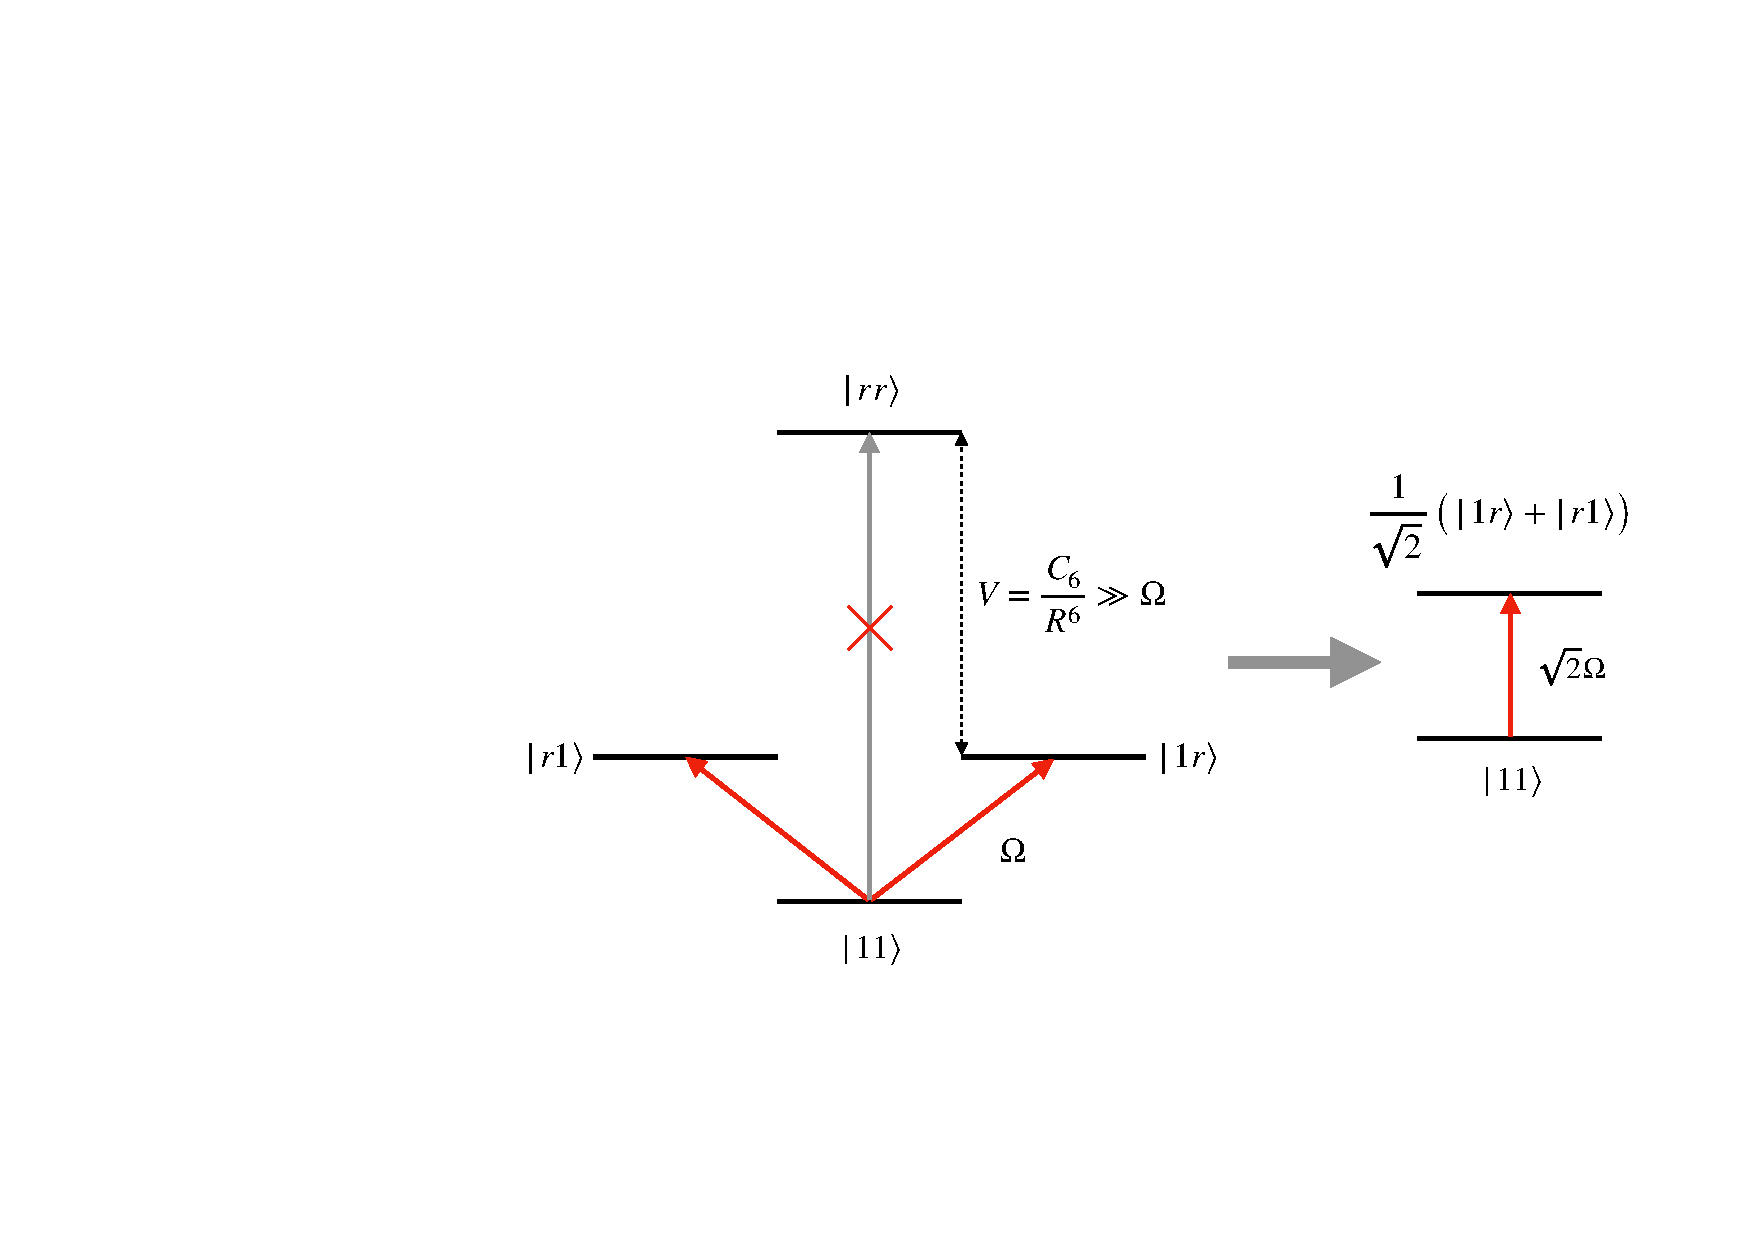
\includegraphics[width=0.75\textwidth]{images/rydberg_blockade_scheme.pdf}
	\caption{За счёт эффекта ридберговской блокады атомы не могут одновременно возбудиться в ридберговское состояние, из-за чего возникают осцилляции между невозбужденным состоянием $\ket{11}$ и суперпозицией $\frac{1}{\sqrt{2}}\left(\ket{1r} + \ket{r1}\right)$, в которой лишь один из атомов находится в ридберговском состоянии.}
	\label{fig:rydberg_blockade}
\end{figure}

Если расстояние между атомами достаточно маленькое, то при одновременном воздействии резонансным полем на переход $\ket{1}\leftrightarrow\ket{r}$ атомы не могут одновременно возбудиться в ридберговское состояние $\ket{rr}$, так как оно сдвинуто по энергии на $V \gg \Omega$. Из-за этого возникают осцилляции Раби между невозбужденным состоянием $\ket{11}$ и суперпозицией $\frac{1}{\sqrt{2}}\left(\ket{1r} + \ket{r1}\right)$, в которой возбужден лишь один из атомов. Характерное расстояние, на которое нужно сблизить атомы, чтобы наблюдался эффект ридберговской блокады, определяется как $R_B = \left(\frac{C_6}{\Omega}\right)^{1/6}$, называется радиусом ридберговской блокады и составляет примерно $10 \;\text{мкм}$ для $\ket{r}=\ket{70 S_{1/2}}$ и $\Omega = 2\pi \times 1 \;\text{МГц}$. Видно, что за счет такого механизма можно приготовить максимально запутанное состояние Бэлла в базисе $\ket{1}, \ket{r}$. Подбором правильной импульсной последовательности можно получить нативный $CZ$ гейт в кубитном базисе за счёт эффекта ридберговской блокады, аналогично можно делать многокубитные гейты \cite{toffoli}, размещая несколько атомов в радиусе ридберговской блокады. Более подробно двухкубитные гейты будут обсуждаться в главе \ref{sec:Chapter_4}.



\textcolor{red}{Можно построить график энергии ридберговского взаимодействия от расстояния между атомами для n=72, например.}



\subsection{Считывание состояния}

\subsection{Цикл работы квантового компьютера на нейтральных атомах}

\textcolor{red}{Вставить сюда характерные времена этапов работы процессора на нейтральных атомах, а также сравнение с другими работами(лучшие результаты) в виде таблицы.}

\newpage